% -*-cap1.tex-*-
% Este fichero es parte de la plantilla LaTeX para
% la realización de Proyectos Final de Carrera, protejido
% bajo los términos de la licencia GFDL.
% Para más información, la licencia completa viene incluida en el
% fichero fdl-1.3.tex

% Copyright (C) 2009 Pablo Recio Quijano 

%\section{Introducción}

A continuación se muestran los resultados del estudio tal y como se describieron en la sección anterior.

\section{Localización de la literatura}
En la tabla \ref{tab:ResumenBusquedaResultados} se muestran las búsquedas realizadas en las bibliotecas digitales más importantes en ciencias de la computación, los términos de búsqueda utilizados, el número de documentos obtenidos. En cada biblioteca, se utilizaron los formularios de búsqueda avanzada.

\begin{table}[H]
  \begin{center}
  \begin{tabular}{| m{3.5cm} | m{6cm} | m{3cm} | c |}
    \hline
    SOURCE & SEARCH TERMS & SEARCH SCOPE & RESULTS\\
    \hline
    \hline
    Wiley Online Library & assessment AND ``generic competences`` OR ``generic skills`` AND (TEL OR ICT OR CBI) & in All Fields & 140 \\
    \hline
    World Scientific Net & ``generic competences`` OR ``generic skills`` AND assessment & Anywhere in article & 20\\
    \hline
    Springer & (``generic skills`` OR ``generic competences``) AND  students AND (TEL OR CBI OR ICT) & All fields (Including full text) & 140\\
    \hline
    ACM Digital Library & (assessment and ``generic skills``) and (TEL or LMS or ICT or CBI) & Any field (title, abstract, review) & 57\\
    \hline
    ACM Digital Library & (assessment and ``generic competences``) and (TEL or LMS or ICT or CBI) & Any field (title, abstract, review) & 15\\
    \hline
    IEEE Digital Library (Xplore) & (((TEL or LMS or ICT or CBI) AND (``generic skills`` OR ``generic competences``)) AND assessment) & Full text and metadata & 48\\
    \hline
    Scopus & (((TEL or LMS or ICT or CBI) AND (``generic skills`` OR ``generic competences``)) AND assessment) & All fields (Including full text) & 47\\
    \hline
    \multicolumn{3}{|r|}{TOTAL} & 467\\
    \hline
  \end{tabular}
\end{center}
\caption{Resumen de búsqueda de bibliografía}
\label{tab:ResumenBusquedaResultados}
\end{table} 


%\section{Selección de trabajos}
%En la tabla \ref{tab:ResumenSelecccionResultados} se muestran los resultados de la clasificación.

En total se recopilaron 467 trabajos, que fueron revisados para identificar si eran de utilidad para el estudio y descartados si cumplían alguno de los criterios de exclusión. El número de estudios primarios resultante (después de aplicar criterios de selección y exclusión) fue de 37 trabajos (casi un 8\% del total de trabajos recopilados). Los resultados de esta clasificación pueden verse e la tabla \ref{tab:ResumenSelecccionResultados}.

\begin{table}[H]
  \begin{center}
  \begin{tabular}{| m{4cm} | c | c |}
    \hline
    CRITERION & STUDIES & FRECUENCY\\
    \hline
    \hline 
    Included & 37 & 7,92\% \\
    \hline
    Off Topic & 402 & 86,08\% \\
    \hline
    Unsupported Language & 1 & 0,21\% \\
    \hline
    Duplicated & 20 & 4,28\% \\
    \hline
    Unread & 7 & 1,50\% \\
    \hline
    Total & 467 & 100\% \\
    \hline
  \end{tabular}
\end{center}
\caption{Resumen de selección de bibliografía}
\label{tab:ResumenSelecccionResultados}
\end{table} 


%\section{Extracción de los datos}
%Se han seleccionado como estudio primario únicamente 37 artículos, un 7,92\% del total de los revisados. Casi la mayor parte de los seleccionados se pueden localizar en los últimos años, entre 2008 y 2013 (Tabla \ref{tab:ResumenAniosResultados} y figura \ref{fig:PublicacionesAnuales}). 

La distribución de la producción de esta selección primaria a lo largo de los años puede verse en la tabla \ref{tab:ResumenAniosResultados} y figura \ref{fig:PublicacionesAnuales}. Casi la mayor parte de los seleccionados se pueden localizar en los últimos años, entre 2008 y 2013.


\begin{table}[H]
  \begin{center}
  \begin{tabular}{| m{4cm} | c |}
    \hline
    YEAR & RESULTS\\
    \hline
    \hline 
    1996 & 0\\
    \hline
    1997 & 1\\
    \hline
    1998 & 0\\
    \hline
    1999 & 0\\
    \hline
    2000 & 0\\
    \hline
    2001 & 0\\
    \hline
    2002 & 0\\
    \hline
    2003 & 0\\
    \hline
    2004 & 0\\
    \hline
    2005 & 2\\
    \hline
    2006 & 2\\
    \hline
    2007 & 2\\
    \hline
    2008 & 11\\
    \hline
    2009 & 2\\
    \hline
    2010 & 3\\
    \hline
    2011 & 6\\
    \hline
    2012 & 8\\
    \hline
    2013 & 12 \\
    \hline
  \end{tabular}
\end{center}
\caption{Resumen de selección de bibliografía}
\label{tab:ResumenAniosResultados}
\end{table} 

La revista es el medio en el que más de este tipo de artículos se han publicado, tal y como se puede consultar en la tabla \ref{tab:ResumenForumResultados} y en la figura \ref{fig:PublicacionesTipos} con un 56,8\% del total.

\begin{figure}[H]
  \begin{center}
    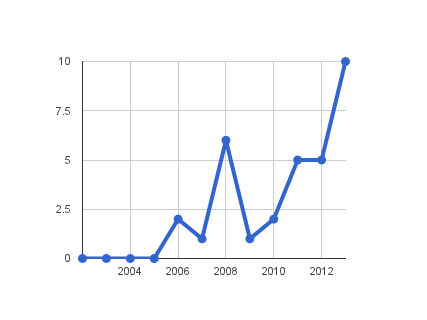
\includegraphics[scale=0.7]{cap3_pub_anuales.png}
  \end{center}
  \caption{Distribución de publicaciones por años}
  \label{fig:PublicacionesAnuales}
\end{figure}

\begin{table}[H]
  \begin{center}
  \begin{tabular}{| m{4cm} | c |}
    \hline
    PUBLICATION TYPE & RESULTS\\
    \hline
    \hline 
    Journal & 21 \\
    \hline
    Conference & 12 \\
    \hline
    Chapter & 4 \\
    \hline
  \end{tabular}
\end{center}
\caption{Resumen de selección de bibliografía}
\label{tab:ResumenForumResultados}
\end{table} 

\begin{figure}[H]
  \begin{center}
    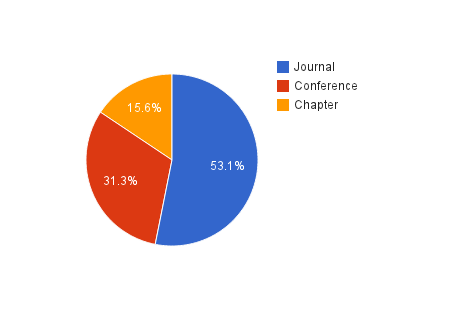
\includegraphics[scale=0.7]{cap3_pub_types.png}
  \end{center}
  \caption{Distribución de publicaciones por tipo}
  \label{fig:PublicacionesTipos}
\end{figure}

La distribución de las publicaciones según el soporte en el que han sido publicados es el que se muestra en la tabla \ref{tab:DistribucionPublicaciones}

\begin{table}[H]
  \begin{center}
  \begin{tabular}{| m{12cm} | c |}
    \hline
    PUBLICATION FORUM & PAPERS\\
    \hline
    \hline 
    World Scientific and Engineering Academy and Society Conferences & 4\\
    \hline
    IEEE Global Engineering Education Conference & 3\\
    \hline
    Australian Society for Computers in Learning in Tertiary Education & 2\\
    \hline
    European Journal of Education & 2\\
    \hline
    Revista Iberoamericana de Tecnologías del Aprendizaje & 2\\
    \hline
    ACM SIGCSE Bulletin & 1\\
    \hline
    Assessment \& Evaluation in Higher Education & 1\\
    \hline
    Australasian Journal of Educational Technology & 1\\
    \hline
    Conference on Software Engineering Education and Training & 1\\
    \hline
    Competency-based Language Teaching in Higher Education & 1\\
    \hline
    Computers in Human Behavior & 1\\
    \hline
    Computing Colombian Conference & 1\\
    \hline
    Decision Support Systems & 1\\
    \hline
    Frontiers in Education Conference & 1\\
    \hline
    Game-based learning in higher education and lifelong learning: bridging the gap between theory and practice & 1\\
    \hline
    Human Factors and Ergonomics in Manufacturing \& Service Industries & 1\\
    \hline
    IFIP Advances in Information and Communication Technology & 1\\
    \hline
    International Conference on Advanced Learning Technologies & 1\\
    \hline
    International Journal of Learning Technology & 1\\
    \hline
    International Review of Education & 1\\
    \hline
    Journal of Computer Assisted Learning & 1\\
    \hline
    Medical Education & 1\\
    \hline
    Research in Higher Education & 1\\
    \hline
    Revista de Educación & 1\\
    \hline
    The Internet and Higher Education & 1\\
    \hline
    Ubiquitous and Mobile Learning in the Digital Age & 1 \\
    \hline
  \end{tabular}
\end{center}
\caption{Distribución de las publicaciones}
\label{tab:DistribucionPublicaciones}
\end{table} 



\section{Extración de datos}

Una vez revisados todos los artículos se han extraído unas características o categorías comunes a la tipología de los trabajos. Todos los trabajos seleccionados hacen uso de algún tipo de software o metodología para evaluar algún tipo de competencia genérica. Pero ningún trabajo utiliza un enfoque como el que se propone en la introducción de este capítulo, es decir, aprovechando los registros de interacción de los estudiantes con el LMS como indicadores del desempeño de las competencias genéricas. Encontramos trabajos que se apoyan en la tecnología para las competencias pero que terminan delegando parte de la evaluación en el alumno, ya sea mediante autoevaluación o evaluación entre iguales. Otros trabajos se basan en videojuegos o en las redes sociales para evaluar alguna competencia, mientras que otros desarrollan algún tipo de software o técnica. Finalmente hay algunos trabajos que simplemente detectan en su entorno la necesidad de la evaluación de las competencias de manera automática porque su forma de hacerlo les ocasiona una serie de problemas o desventajas con respecto a otro método que proponen o demandan. Además se han encontrado algunas revisiones sobre la literatura relacionadas que también serán tratadas a parte.  En la tabla \ref{tab:PublicacionesForum} se puede ver la distribución de las publicaciones, apoyadas gráficamente en la figura  \ref{fig:PublicacionesForum}.

\begin{table}[H]
  \begin{center}
  \begin{tabular}{| m{4cm} | c |}
    \hline
    PUBLICATION ISSUE & PAPERS\\
    \hline
    \hline 
    Evaluaciones & 10\\
    \hline
    Necesidad & 8\\
    \hline
    Red social & 2\\
    \hline
    Videojuegos & 5\\
    \hline
    Revisiones & 3\\
    \hline
    Técnicas & 9 \\
    \hline
  \end{tabular}
\end{center}
\caption{Distribución de publicaciones por tratamiento del problema}
\label{tab:PublicacionesForum}
\end{table} 

\begin{figure}[H]
  \begin{center}
    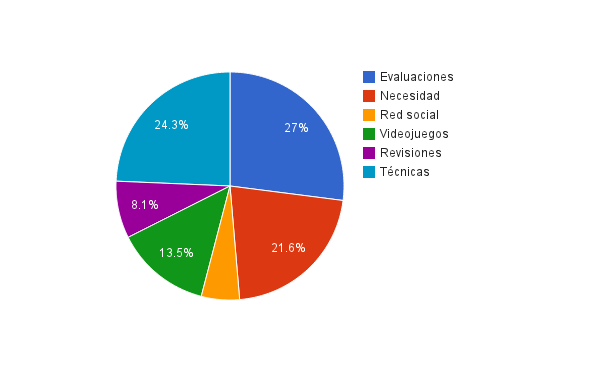
\includegraphics[scale=0.7]{cap3_pub_forum.png}
  \end{center}
  \caption{Distribución de publicaciones por tratamiento del problema}
  \label{fig:PublicacionesForum}
\end{figure}
